\documentclass{article}%
\usepackage[T1]{fontenc}%
\usepackage[utf8]{inputenc}%
\usepackage{lmodern}%
\usepackage{textcomp}%
\usepackage{lastpage}%
\usepackage[head=40pt,margin=0.5in,bottom=0.6in]{geometry}%
\usepackage{graphicx}%
%
\title{\textbf{Cinco presos han muerto en lo que va de año en calabozos de la PNB}}%
\author{El Nacional Web}%
\date{22/10/2018}%
%
\begin{document}%
\normalsize%
\maketitle%
\textbf{URL: }%
http://www.el{-}nacional.com/noticias/sucesos/cinco{-}presos{-}han{-}muerto{-}que{-}ano{-}calabozos{-}pnb\_256744\newline%
%
\textbf{Periodico: }%
EN, %
ID: %
256744, %
Seccion: %
Sucesos\newline%
%
\textbf{Palabras Claves: }%
PNB, Sociedad\newline%
%
\textbf{Derecho: }%
1.2, %
Otros Derechos: %
, %
Sub Derechos: %
1.2.4\newline%
%
\textbf{EP: }%
NO\newline%
\newline%
%
\textbf{\textit{Las causas de dichas muertes según versiones de familiares, se debe a golpes recibidos por sus propios compañeros y un caso de desnutrición~}}%
\newline%
\newline%
%
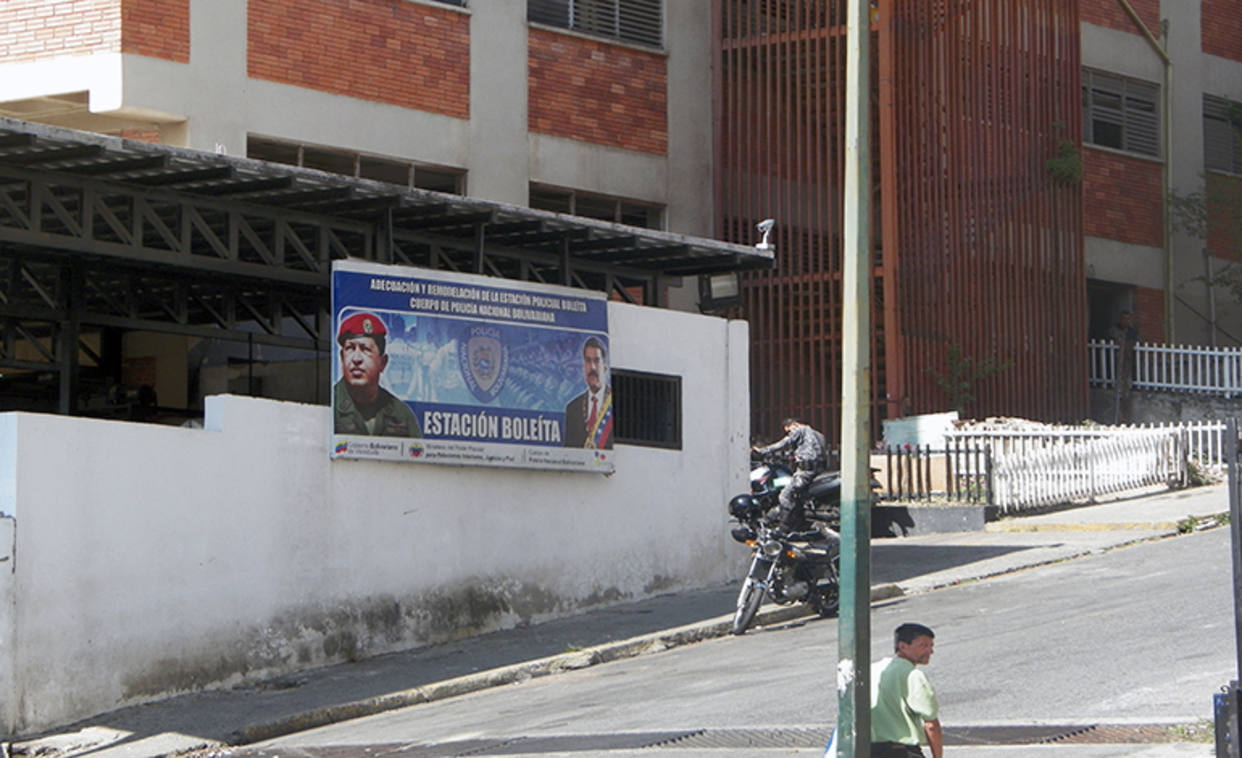
\includegraphics[width=300px]{125.jpg}%
\newline%
%
Cinco presos han muerto en lo que va de año en dos centros de detención preventiva de la Policía Nacional Bolivariana (PNB) en Caracas, específicamente en San Agustín y Boleíta, en la conocida zona 7 de la policía metropolitana.%
\newline%
%
El Observatorio Venezolano de Prisiones (OVP) registró que desde~abril hasta octubre~cinco los privados de libertad fallecieron dentro de los recintos penitencirios. La organización destacó que hasta el momento no existen reponsables del hecho ni un pronunciamiento del Estado.%
\newline%
%
El primer crimen fue cometido el 28 de abril en Boleíta, los detenidos ahorcaron a Carlos Enrique Pérez Gómez (21), según relataron los propios familiares, el preso habría defecado dentro del calabozo y por eso sus compañeros lo mataron.%
\newline%
%
Carlos Francisco Rangel Novais (27), fue la segunda víctima quien el 16 de julio fue sacado sin vida de los calabozos de la PNB de San Agustín, los funcionarios le dijeron a los familiares que había sostenido una riña con los compañeros sin dar más explicación. Sus familiares, quienes habían visto al preso un día antes, notaron marcas en su cuello y muñecas, además el joven les explicó que estaba siendo torturado por los funcionarios.%
\newline%
%
Ronald Daniel Subero Alcalá, fue asesinado el 7 de agosto, se convirtió en el segundo preso fallecido de Boleíta, este hombre fue golpeado por sus compañeros y sacado sin vida.%
\newline%
%
El cuarto reporte fue el de Carlos Suárez Navarro (21), ~falleció el 15 de octubre. Tenía 40 días detenido en los calabozos de San Agustín y según relató el propio interno a su familia este no ingería alimentos a pesar que su familia se la llevaba nunca le llegaban a sus manos, por lo que había rebajado considerablemente, presentando un estado de desnutrición y finalmente falleció.%
\newline%
%
El último reporte que tiene OVP, es el deceso Kenry Joseth Bogado Hernández (33), se pudo conocer que falleció en los calabozos de San Agustín este domingo 21 de octubre, según conoció esta organización habrían sido sus compañeros de celda, al menos siete que lo golpearon.%
\newline%
%
Con información de nota de prensa%
\newline%
%
\end{document}